\documentclass[a4paper]{article}
\usepackage{graphicx}
\usepackage{amsmath}
\usepackage{amsthm}
\usepackage{listings}
\usepackage{xcolor}
\usepackage{geometry}
\usepackage{hyperref}
\usepackage{marginnote}

\newgeometry{margin=1in}
\setcounter{section}{-1}

\theoremstyle{definition}
\newtheorem{example}{Example}
\newtheorem{definition}{Definition}


\lstset{language=python, basicstyle=\ttfamily\small, 
        keywords={import, as, linspace, normal, rand, sum, print, f, for, in},
        keywordstyle=\color{purple}, commentstyle=\color{gray}, stringstyle=\color{blue}, showstringspaces=false}

\title{An Introduction to Regression Neural Networks}
\author{Moaaz Abo-Shaeer}
\date{}
\begin{document}
\maketitle

\section{Background}
"AI" and Machine learning are quite hot topics, and it may not be obvious what they actually are. Machine learning is often classified into \textit{supervised} and \textit{unsupervised} learning.
Supervised algorithms learn from data that has been labeled\footnote{\textit{Labeled} data is data that's associated with a correct answer, e.g., images of people which have the labels "male" or "female" provided to a model which learns to differentiate men from women.} by humans, while unsupervised algorithms attempt to find patterns on their own.\\
Supervised machine learning can be classified into \textit{classification} and \textit{regression}.
Classification is where the algorithm is given data and asked to classify it into discrete categories (e.g. photos in your phone classified into folders for each person), while regression is basically function approximation, where an algorithm is given data points and provides the general trend that this data follows allowing it to predict values for new data points.
This introduction focuses on neural networks used in regression.

\section{Simple Linear Regression}
If we know that our data has a linear trend then we know it must follow the equation $y = wx + b$, our task now is simply to find $w$ and $b$, called the \textbf{\textit{weight}} and \textbf{\textit{bias}} respectively.
There is an analytical solution to this specific problem, but it doesn't scale to other cases so we will use a more numerical solution that can pave the way to neural networks.
We must first find a metric to evaluate our regression line which we'll refer to as the \textit{loss function}, our metric will be the mean squared error (MSE).

\begin{definition}{Mean Squared Error}
    is defined as:
    \begin{equation*}
        E = \frac{1}{n} \sum_{i=1}^{n} (y_i - \hat{y}_i)^2 = \frac{1}{n} \sum_{i=1}^{n} (y_i - (wx_i + b))^2
    \end{equation*}
    Where $y_i$ is an actual data point and $\hat{y}_i = wx_i + b$ is the prediction of our model.
\end{definition}
\noindent
Now we can tweak $w$ and $b$ and then evaluate the model using MSE, by repeating these two steps, we can minimize the error of our model.

\subsection{Gradient Descent}
Let $\Delta w$ and $\Delta b$ be the tweaks we apply to our parameters.
Since we've used MSE, we know that the error follows parabolic curves with varying $w$ or $b$.
So by observing the rate of change of the error function with respect to our parameters we find that the further we are from the minimum error the greater the slope is, which can be used to indicate \textit{how much} we should tweak our parameter.
We also find that if the rate of change is positive, then we must decrease our parameter ($w$ or $b$) to move towards the minimum and vice versa.
Therefore, $\Delta w \propto -\frac{\partial E}{\partial w}$ and $\Delta b \propto -\frac{\partial E}{\partial b}$.
Knowing this, we can tweak our parameters for multiple iterations to minimize error.
\begin{align*}
    w' = w + \Delta w &= w -\eta \frac{\partial E}{\partial w} = w + \frac{2\eta}{n} \sum_{i=1}^{n} (y_i - (wx_i + b))x_i \\
    b' = b + \Delta b &= b -\eta \frac{\partial E}{\partial b} = b + \frac{2\eta}{n} \sum_{i=1}^{n} (y_i - (wx_i + b))
\end{align*}
\noindent
Where $\eta$ is a constant of proportionality called the \textit{learning rate}.\\
And the iterative algorithm we just described is called \textit{gradient descent}, where each iteration over the data is called an \textit{epoch}.

\begin{example}[Simple Linear Regression Code]
    A simple example code of linear regression using gradient descent.
    \begin{lstlisting}
import matplotlib.pyplot as plt
import numpy as np

X = np.linspace(-10, 10, 50) # 50 evenly spaced numbers between -10 and 10
Y = 0.3 * X + 1 + np.random.normal(0, 1, size=X.shape) # y = 0.3x + 1 + noise

w = np.random.rand()
b = np.random.rand()

eta = 2e-4 # Learning rate
for epoch in range(3):
    w += 2 * eta * np.sum((Y - (w * X + b)) * X)
    b += 2 * eta * np.sum(Y - (w * X + b))

Yhat = w * X + b # Predictions

print(f'Final weights: w = {w}, b = {b}')
    \end{lstlisting}
\end{example}

\begin{figure}[h]
    \centering
    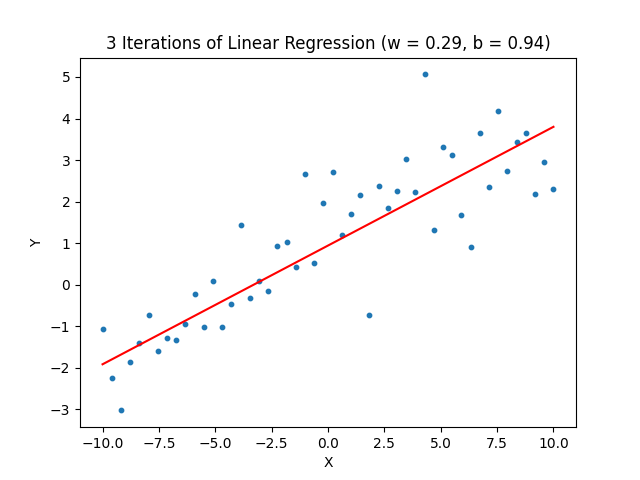
\includegraphics[width=0.5\textwidth]{Media/simple_linear_regression.png}
    \caption{The original data points (blue) following the trend y = 0.3x + 1, and the regression line (red) after 3 iterations of gradient descent over the data set.}
    \label{fig:simple_linear_regression}
\end{figure}


\section{More Complex Models}
Previously, we only discussed scalar single variable models used for regression, and the solution we found may have seemed overkill for the a problem with a known analytical solution.
But we can apply the same method to models with multiple inputs and outputs as discussed in the next sections.
\subsection{Multivariable Linear Regression}
If the value we are trying to predict depends linearly on multiple variables, our model becomes $y = w_1x_1 + w_2x_2 + ... + w_nx_n + b$.
But we can still use gradient descent to minimize error.
\begin{align*}
    w_k' = w_k + \Delta w &= w_k -\eta \frac{\partial E}{\partial w} = w_k + \frac{2\eta}{n} \sum_{i=1}^{n} (y_i - \hat{y}_i)x_{k,i} \\
    b_k' = b_k + \Delta b &= b_k -\eta \frac{\partial E}{\partial b} = b_k + \frac{2\eta}{n} \sum_{i=1}^{n} (y_i - \hat{y}_i)
\end{align*}
\noindent
Notice that $i$ is the index of the data point while $k$ is the index of the term in the model.

\subsection{Vector-valued Linear Regression}
In the previous section, we considered a model with multiple inputs.
Now we can find a Model with $n$ inputs and $m$ outputs called \text{vector-valued linear regression}\footnote{Also called multivariate linear regression, but I used this name to prevent confusion}.

\begin{equation*}
    \begin{bmatrix} y_1\\ y_2\\ ...\\ y_m \end{bmatrix} = \begin{bmatrix} w_{1,1} & w_{1,2} & ... & w_{1,n}\\ w_{2,1} & w_{2,2} & ... & w_{2,n}\\ ... & ... & ... & ...\\ w_{m,1} & w_{m,2} & ... & w_{m,n} \end{bmatrix} \begin{bmatrix} x_1\\ x_2\\ ...\\ x_n \end{bmatrix} + \begin{bmatrix} b_1\\ b_2\\ ...\\ b_m \end{bmatrix}
\end{equation*}
Notice that for a single $y_i$ the model has the same equation as multivariable linear regression, it's only more concise to use linear algebra in this case, we can write the same equation in much shorter form.
\begin{equation*}
    \vec{y} = W \vec{x} + \vec{b}
\end{equation*}

\subsection{Polynomial Regression}
If the data doesn't follow a linear trend, we must use a non-linear model to approximate it.
And the easiest non-linear model is an $n$th-degree polynomial $y = b + w_1x + w_2x^2 + ... + w_nx^n$.
We can still use MSE and gradient descent, but the gradient descent equations for the weights are slightly different.
\begin{equation*}
    w_k' = w_k + \Delta w = w_k -\eta \frac{\partial E}{\partial w} = w_k + \frac{2\eta}{n} \sum_{i=1}^{n} (y_i - \hat{y}_i)\cdot kx^{k-1} \\
\end{equation*}

\section{Regression Neural Networks}
To approximate non-linear data, we can use multiple stages of vector-valued linear regression with some non-linear function added between them.
That is the basic structure of a regression neural network.

\subsection{ReLU and Activation Functions}
If our model only consists of multiple stages of linear functions it will also produce a linear function, so if we want the model to approximate non-linear data we must add a non-linear function between these stages.
Activation functions are these non-linear functions, the most common example for regression is ReLU (Rectified Linear Unit) which is just a ramp function $ReLU(x) = \max(0, x)$.
But the linear transformations preceding and following it can bend it to fit the data.
Let's use simple linear equations as an example.

\begin{example}[ReLU Example]
    If the first stage is $z = w_1 x + b_1$, the second stage is the ReLU function $a = ReLU(z) = \max(0, z)$, and the third stage is $\hat{y} = w_2 a + b_2$, then the full model is
    \begin{equation*}
        \hat{y} = w_2 ReLU(w_1 x + b_1) + b_2
    \end{equation*}
    Notice that $w_1$ produces x axis scaling, $b_1$ produces x axis translation, $w_2$ produces y axis scaling, and $b_2$ produces y axis translation.
    These parameters can optimized to make the model fit the data, and if we can add multiple similar functions we can produce more complex non-linear models.\\
    The stages in a neural network are called \textit{layers}\footnote{The first and second stage are considered one layer since applying the activation function isn't usually a separate stage}, and the internal stages which produce $z$ and $a$ are called \textit{hidden layers}.
\end{example}

\begin{figure}[h]
    \centering
    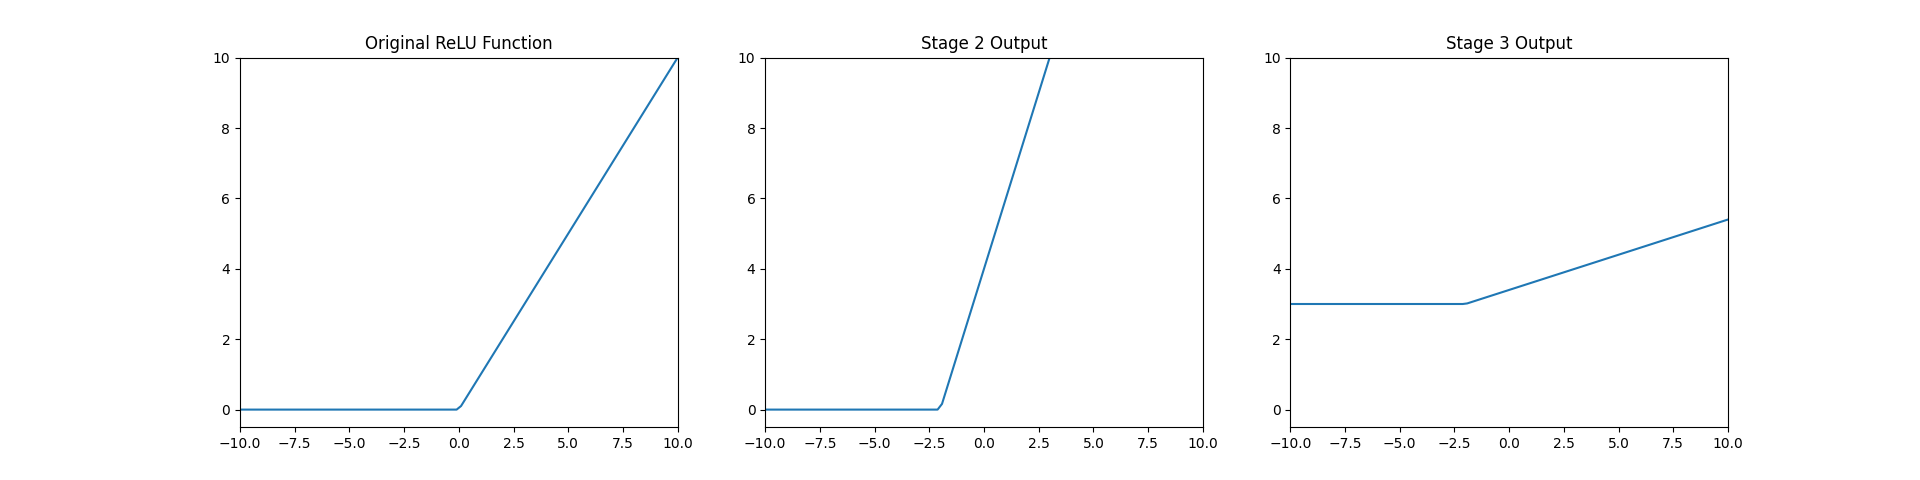
\includegraphics[width=1\textwidth]{Media/ReLU.png}
\end{figure}
\pagebreak

\subsection{The Structure of a Neural Network}
Let us consider a general neural network with multiple inputs in an input vector called \textit{the input layer} $\vec{x}$, the first layer consists of a weight matrix $W^1$, a bias vector $\vec{b}^1$ and an activation function $f^1$.
\begin{equation*}
    \vec{a}^1 = f^1(\vec{z}^1) = f^1 \left(W^1 \vec{x} + \vec{b}^1\right)
\end{equation*}
The vector $\vec{a}^1$ is called \textit{activation} and it's the output of the first layer, and the vector $\vec{z}^1$ is called \textit{pre-activation} and it's the output of the linear transformation before the activation function.
The second layer takes $\vec{a}^1$ as input and has a similar equation.
\begin{equation*}
    \vec{a}^2 = f^2(\vec{z}^2) = f^2 \left(W^2 \vec{a}^1 + \vec{b}^2\right)
\end{equation*}
In a classification neural network, the output usually uses an activation function like \href{https://en.wikipedia.org/wiki/Softmax_function}{softmax} or \href{https://en.wikipedia.org/wiki/Sigmoid_function}{sigmoid}.
But in regression the output layer may not have an activation function at all.
\begin{equation*}
    \hat{\vec{y}} = W^3 \vec{a}^2 + \vec{b}^3
\end{equation*}

\subsection{Backpropagation}

Notice that in \textbf{Example 2} that the presence of the activation function will make the calculation of $\frac{\partial E}{\partial w_i}$ or $\frac{\partial E}{\partial b_i}$ more complex.
So we will have to use the chain rule to get the partial derivatives of the error with respect to the parameters, applying the chain rule backward throughout the whole model is the \textit{backpropagation} algorithm.
\subsubsection{Hadamard Product}
Multiplying two vectors element-wise is called the \textit{Hadamard product} and is denoted by $\odot$, where the main difference between it and the dot product is that the output of the Hadamard product is also a vector.
\begin{equation*}
    \begin{bmatrix} a_1\\ a_2\\ ...\\ a_n \end{bmatrix} \odot \begin{bmatrix} b_1\\ b_2\\ ...\\ b_n \end{bmatrix} = \begin{bmatrix} a_1 b_1\\ a_2 b_2\\ ...\\ a_n b_n \end{bmatrix}
\end{equation*}
\vspace{10pt}

\begin{example}[Backpropagation Example]
    There are quick formulas to apply backpropagation automatically, but we will first do it by hand on a small neural network as an example.
    
    \noindent
    Using the standard notation, we place the layer number as a superscript on the parameters.\\
    In a two-layer neural network, if the first layer is 
    \begin{equation}
        \begin{bmatrix} z_1\\ z_2 \end{bmatrix} = \begin{bmatrix} w^{1}_{1} \vspace{2pt}\\ w^{1}_{2} \end{bmatrix} x + \begin{bmatrix} b^{1}_1 \vspace{2pt}\\ b^{1}_2 \end{bmatrix}
    \end{equation}
    with the ReLU function applied to it
    \begin{equation}
        \begin{bmatrix} a_1\\ a_2 \end{bmatrix} = ReLU\left(\begin{bmatrix} z^1_1 \vspace{2pt}\\ z^1_2 \end{bmatrix}\right) = \begin{bmatrix} \max(0, z_1)\\ \max(0, z_2) \end{bmatrix}
    \end{equation}
    and the second (layer without an activation function) is
    \begin{equation}
        \hat{y} = \begin{bmatrix} w^{2}_{1} & w^{2}_{2} \end{bmatrix} \begin{bmatrix} a_1\\ a_2 \end{bmatrix} + b^{2}_1 = w^{2}_{1} a_1 + w^{2}_{2} a_2 + b^{2}_1
    \end{equation}
    We need to differentiate the error with respect to the parameters, and we know that $\frac{\partial E}{\partial w^2_i} = \frac{\partial E}{\partial \hat{y}} \cdot \frac{\partial \hat{y}}{\partial w^2_i}$ and $\frac{\partial E}{\partial b^2_i} = \frac{\partial E}{\partial \hat{y}} \cdot \frac{\partial \hat{y}}{\partial b^2_i}$, but $\frac{\partial \hat{y}}{\partial b^2_1} = 1$.\\
    For the weights, we use the chain rule on the error function to get $\frac{\partial E}{\partial \hat{y}} = \frac{2}{n} \sum_{i=1}^{n} (y_i - \hat{y}_i)$.
    Then, from \textbf{Eq. (3)} we find that $\frac{\partial \hat{y}}{\partial w^2_i} = a_i$.
    Therefore,
    \begin{equation}
        \begin{bmatrix} \frac{\partial E}{\partial w^{2}_{1}} \vspace{4pt}\\ \frac{\partial E}{\partial w^{2}_{2}} \end{bmatrix} = \frac{\partial E}{\partial \hat{y}} \begin{bmatrix} a_1\\ a_2\end{bmatrix}, \quad \frac{\partial E}{\partial b^{2}_1} = \frac{\partial E}{\partial \hat{y}}
    \end{equation}
    \vspace{5pt}
    \\
    From \textbf{Eq. (1)} and \textbf{Eq. (2)} we know that $\frac{\partial E}{\partial w^1_i} = \frac{\partial E}{\partial a_i} \cdot \frac{\partial a_i}{\partial z_1} \cdot \frac{\partial z_1}{\partial w^1_i}$.
    Then by looking at \textbf{Eq. (3)}, $\frac{\partial E}{\partial a_i} = \frac{\partial E}{\partial \hat{y}} \cdot w^2_i$, from \textbf{Eq. (2)} we find that $\frac{\partial a_i}{\partial z_i} = ReLU'(z_i)$, and from \textbf{Eq. (1)} we find that $\frac{\partial z_i}{\partial w^1_i} = x$.
    Therefore,
    \begin{equation}
        \begin{bmatrix} \frac{\partial E}{\partial w^{1}_{1}} \vspace{4pt}\\ \frac{\partial E}{\partial w^{1}_{2}} \end{bmatrix} = \frac{\partial E}{\partial \hat{y}} \begin{bmatrix} w^2_1 \vspace{2pt}\\ w^2_2\end{bmatrix} \odot \begin{bmatrix} ReLU'(z_1)\\ ReLU'(z_2) \end{bmatrix} \cdot x,
        \quad \begin{bmatrix} \frac{\partial E}{\partial b^{1}_{1}} \vspace{4pt}\\ \frac{\partial E}{\partial b^{1}_{2}} \end{bmatrix} = \frac{\partial E}{\partial \hat{y}} \cdot \begin{bmatrix} w^2_1 \vspace{2pt}\\ w^2_2\end{bmatrix} \cdot \begin{bmatrix} ReLU'(z_1)\\ ReLU'(z_2) \end{bmatrix}
    \end{equation}
    Where the derivative of the ReLU function $ReLU'(z_i) = \begin{cases} 1 & z_i > 0 \vspace{-3pt} \\ 0 & z_i \leq 0 \end{cases}$.
\end{example}
\noindent

\subsection[Generalised Backpropagation Formulas]{Generalised Backpropagation Formulas\footnote{These formulas will not be properly explained here, if you want a better understanding of them I would recommend reading \href{http://neuralnetworksanddeeplearning.com/chap2.html}{Chapter 2 of Neural Networks and Deep Learning by Michael Nielsen} and watch \href{https://youtu.be/Ilg3gGewQ5U?si=vHY4JfwTyA1r0Q89}{Backpropagation, intuitively by 3Blue1Brown} for intuition.}}
Now we can look at the standard formulas of backpropagation.
Consider a neural network with $L$ layers, with weight matrices $W^l$ and bias vectors $\vec{b}^l$, each layer with an activation function $f^l$, and let $z^l_{j}$ and $a^l_{j}$ be the pre-activations and activations respectively.
The vector $\delta^l$ contains the partial derivatives of the error with respect to the pre-activations of layer $l$, which means that
\begin{equation}
    \delta^l_j = \frac{\partial E}{\partial z^l_j}
\end{equation}
\noindent
Therefore, the vector $\delta^L$ of the last layer is
\begin{equation}
    \delta^L = \frac{\partial E}{\partial a^L} \odot \frac{\partial a^L}{\partial z^L} = \frac{\partial E}{\partial a^L} \odot f'^L(z^L)
\end{equation}
For the hidden layers we have
\begin{equation}
    \delta^l = (W^{l+1})^T \delta^{l+1} \odot f'^l(z^l)
\end{equation}

\noindent
And the partial derivatives of the error with respect to the weights and biases of each layer are
\begin{equation*}
    \frac{\partial E}{\partial w^l_{j,k}} = \frac{\partial E}{\partial z^l_{j}} \cdot (a^{l-1}_{k}), \quad \frac{\partial E}{\partial b^l_{j}} = \frac{\partial E}{\partial z^l_{j}}
\end{equation*}
And the vector form of these equations is as follows
\begin{equation*}
    \frac{\partial E}{\partial W^l} = \delta^l (a^{l-1})^T, \quad \frac{\partial E}{\partial \vec{b}^l} = \delta^l
\end{equation*}


\end{document}